\documentclass[10pt, a4paper, oneside, fontset=none]{ctexart}
%调用宏包
\usepackage{amsmath, amsthm, amssymb, graphicx, wrapfig, mathrsfs, upgreek}
\usepackage[bookmarks=true, colorlinks, citecolor=blue, linkcolor=black]{hyperref}
\usepackage{color, framed, geometry, tcolorbox, multirow, booktabs}
\tcbuselibrary{breakable}%box跨页
\tcbuselibrary{skins}%box跨页不留边
%\usepackage{CJKpunct}
\usepackage{marginnote}
\usepackage{makecell, booktabs, longtable}
\usepackage[font=sf, labelfont+=bf]{caption}
\usepackage[font={small, sf}]{subfig}
\usepackage{multicol}
\usepackage{arydshln, nicematrix}%矩阵
\usepackage{extarrows}
\usepackage[american, cuteinductors, ]{circuitikz}
\usepackage{xpatch}
\usepackage{rotating}%旋转
\usepackage{physics}
\usepackage{siunitx}
\usepackage{enumitem}
\usepackage{listings}
\usepackage{dashrule}
\usepackage{tablefootnote}%表格脚注
\usepackage[text=\includegraphics{C:/Users/16870/.vscode/LaTeX_Application/tex/THUEE23-23Autumn/图标简稿.png},angle=0]{draftwatermark}%水印
%\usepackage{tikz}
%基本字体设置
\usepackage[math-style=ISO, bold-style=ISO]{unicode-math}
\setmainfont{KpRoman}
%\setmainfont{EB Garamond}
%\setmathfont{Garamond-Math.otf}[StylisticSet={7,9}]
\setmonofont{Iosevka}
\setmathfont{KpMath-Regular.otf}%NewCMMath-Regular
%\setmathfont[range=bb]{TeXGyrePagellaMath-Regular}
%\setmathsfont(Digits,Latin){Garamond MT Pro}
\setmathfont[range={\int}]{NewCMMath-Regular}
\setCJKmainfont{FZXSSK.TTF}[BoldFont={SourceHanSerifCN-Bold.otf}, ItalicFont={FZXKTK.TTF}, BoldItalicFont={汉仪颜楷W.ttf}]
\setCJKsansfont{汉仪文黑-45W.ttf}[BoldFont={汉仪文黑-75W.ttf}, ItalicFont={FZYanZQKSJF.TTF}]
\setCJKmonofont{LXGWNeoXiHei.ttf}
%附加字体设置
\newCJKfontfamily{\kaico}{可口可乐在乎体 楷体Coca-ColaCareFontKaiTi.TTF}
\newCJKfontfamily{\kai}{FZXKTK.TTF}[BoldFont={汉仪颜楷W.ttf}, ItalicFont={方正清刻本悦宋 简繁.TTF}, BoldItalicFont={FZYanZQKSJF.TTF}]
\newCJKfontfamily{\yan}{方正清刻本悦宋 简繁.TTF}[ItalicFont={FZYanZQKSJF.TTF}]
\newCJKfontfamily{\xiu}{方正宋刻本秀楷_GBK.TTF}[ItalicFont={方正宋刻本秀楷_GBK.TTF}, BoldFont={FZYanZQKSJF.TTF}]
\newCJKfontfamily{\run}{汉仪润圆-45W.ttf}[BoldFont={汉仪润圆-75W.ttf}, ItalicFont={汉仪润圆-45W.ttf}]
\newCJKfontfamily{\wen}{汉仪文黑-45W.ttf}[BoldFont={汉仪文黑-75W.ttf}, ItalicFont={hk4e_zh-cn.ttf}]
%文档格式
\geometry{left=2.24cm, right=2.24cm, top=3.18cm, bottom=3.18cm}
\linespread{1.4}
\numberwithin{equation}{section}
\setcounter{tocdepth}{3}
\setcounter{secnumdepth}{4}
\renewcommand{\theparagraph}{\hskip2em\Alph{paragraph})}
\newcommand{\Section}[1]{ \refstepcounter{section} \section*{*\thesection\texorpdfstring{\quad}{} #1} \addcontentsline{toc}{section}{\makebox[0pt][r]{*}\thesection\texorpdfstring{\quad}{} #1} }
\newcommand{\Subsection}[1]{ \refstepcounter{subsection} \subsection*{*\thesubsection\texorpdfstring{\quad}{} #1} \addcontentsline{toc}{subsection}{\makebox[0pt][r]{*}\thesubsection\texorpdfstring{\quad}{} #1} }
\newcommand{\Subsubsection}[1]{ \refstepcounter{subsubsection} \subsubsection*{*\thesubsubsection\texorpdfstring{\quad}{} #1} \addcontentsline{toc}{subsubsection}{\makebox[0pt][r]{*}\thesubsubsection\texorpdfstring{\quad}{} #1} }
\setlist[itemize]{leftmargin=3em, labelsep=0.25em, itemindent=0em, itemsep=0pt, parsep=0pt, topsep=3pt, partopsep=0pt}
\setlist[description]{align=left, leftmargin=2em, itemindent=-1em, labelsep=1em, parsep=0pt, topsep=3pt, partopsep=0pt}
\setlength{\marginparwidth}{8em}
\setlength{\lineskip}{5pt}
\setlength{\lineskiplimit}{5pt}

\setlength{\abovecaptionskip}{0.3em}
\setlength{\belowcaptionskip}{0em}
\captionsetup[subfigure]{captionskip=0.5em, nearskip=0em}
\captionsetup[table]{justification=raggedright,singlelinecheck=false}
\renewcommand{\thefigure}{\thesection.\arabic{figure}}
\renewcommand{\thetable}{\thesection.\arabic{table}}

\tikzset{every node/.style={scale=0.8}}
\ctikzset{monopoles/vcc/arrow={Stealth[width=4pt, length=6pt]}}
\ctikzset{monopoles/vee/arrow={Stealth[width=4pt, length=6pt]}}
\ctikzset{bipoles/length=1cm} %电路图大小标的
\ctikzset{resistors/thickness=2.5}
\ctikzset{voltage=raised}
\ctikzset{bipoles/cuteswitch/thickness=0.4}
\tikzset{ %元件着色
    R/.append style={color=balib},
    C/.append style={color=balib},
    L/.append style={color=balib},
    Do/.append style={color=balib},
    zDo/.append style={color=balib},
    leDo/.append style={color=balib},
    pDo/.append style={color=balib},
    battery1/.append style={color=meihong!75!black},
    battery2/.append style={color=meihong!75!black},
    battery/.append style={color=meihong!75!black},
    cI/.append style={color=meihong!75!black},
    I/.append style={color=meihong!75!black},
    cV/.append style={color=meihong!75!black},
    V/.append style={color=meihong!75!black},
}
\tikzset{bcirc/.style={circ, color=black}}
\tikzset{wcirc/.style={ocirc, color=black, fill=white}}
\ctikzset{
	*-*/.style = {bipole nodes={bcirc}{bcirc}},
	-*/.style = {bipole nodes={none}{bcirc}},
	*-/.style = {bipole nodes={bcirc}{none}},
	o-o/.style = {bipole nodes={wcirc}{wcirc}},
	-o/.style = {bipole nodes={none}{wcirc}},
	o-/.style = {bipole nodes={wcirc}{none}},
	o-*/.style = {bipole nodes={wcirc}{bcirc}},
	*-o/.style = {bipole nodes={bcirc}{wcirc}}
}
\ctikzset{logic ports=ieee}
\newcommand{\bi}[1]{% name
	\node [currarrow, color=black, anchor=center,
	rotate=\ctikzgetdirection{#1-Iarrow}] at (#1-Ipos) {};
}
\newcommand{\bv}[1]{% name
	\draw [color=black] (#1-Vfrom) .. controls (#1-Vcont1)
	and (#1-Vcont2).. (#1-Vto) node [currarrow,
	sloped, anchor=tip, allow upside down,pos=1]{};
}
\renewcommand{\bf}[1]{% name
	\draw [color=black] (#1-Ffrom) -- (#1-Fto) node [currarrow,
	sloped, anchor=tip, allow upside down,pos=1]{};
}
\ctikzset{!vi/.style={no v symbols, no i symbols, no f symbols}}
%\punctstyle{kaiming}
%定理环境
\theoremstyle{plain}
\newtheorem{theorem}{定理}[subsection]
\newtheorem{definition}{定义}[subsection]
\newtheorem{lemma}[theorem]{引理}
\newtheorem{corollary}[theorem]{推论}
\newtheorem{proposition}[theorem]{命题}

\theoremstyle{definition}
\newtheorem{examplein}[theorem]{\run 例题}
\newtheorem{circum}[theorem]{情形}

\newcommand{\exampleparameter}{0}
\newenvironment{example}[1][0]{% 0/1: no space; 2/3: 5pt space
	\renewcommand{\exampleparameter}{#1}
	\ifnum \exampleparameter>1
		\vspace{10pt}
	\fi
	\hrule
	\vspace{3pt}
	\noindent\hdashrule{\linewidth}{0.5pt}{2pt}
	\vspace{-2em}
	\begin{examplein}
}{% 0/2: -0.5pt space; 1/3: 5pt space
	\end{examplein}
	\vspace{-1em}
	\noindent\hdashrule{\linewidth}{0.5pt}{2pt}\vspace{3pt}
	\hrule
	\ifnum 1=\exampleparameter
		\vspace{10pt}
	\else
		\ifnum 3=\exampleparameter
			\vspace{10pt}
		\else
			\vspace{-0.5pt}
		\fi
	\fi
}

\newenvironment{proofs}[1][\small\proofname]{\begin{pf}[breakable, enhanced jigsaw]\begin{proof}[#1]\small\kai
	\abovedisplayskip=2pt
	\belowdisplayskip=2pt
}{\end{proof}\end{pf}}
\newenvironment{solution}[1][解]{\begin{proofs}[\small\textit{\yan #1}]\renewcommand{\qedsymbol}{$\circledS$}}{\end{proofs}}
\renewcommand{\proofname}{\yan{证明}}

\renewenvironment{cases}[1][l]{\left\{\,\begin{NiceArray}{#1}}{\end{NiceArray}\right.}
%颜色命名
\definecolor{meihong}{rgb}{0.85,0.2,0.47}
\definecolor{bali}{rgb}{0.2,0.6,0.78}
\definecolor{qinglv}{rgb}{0,0.35,0.32}
\definecolor{meihongb}{rgb}{0.85,0.2,0.47}
\definecolor{balib}{rgb}{0.15,0.45,0.58}
\definecolor{qinglvb}{rgb}{0,0.35,0.32}
%box环境
\newtcolorbox{pr}[2][]
{colback=black!5!white,colframe=white!75!black,fonttitle=\sffamily\wen\bfseries,title=#2,#1}
\newtcolorbox[use counter=definition,number within=subsection]{defi}[2][]
{colback=bali!5!white,colframe=bali!75!black,fonttitle=\sffamily\wen\bfseries,title=定义~\thetcbcounter. #2,#1}
\newtcolorbox[auto counter,number within=section]{compl}[2][]
{colback=bali!5!white,colframe=bali!65!black,fonttitle=\sffamily\wen\bfseries,label=#2,title=元件~\thetcbcounter. #2,#1, fontupper=\kai, fontlower=\kai}
\newtcolorbox[use counter=theorem,number within=subsection]{theo}[2][]
{%grow to right by=3.2cm,
colback=meihong!5!white,colframe=meihong!75!black,fonttitle=\sffamily\wen\bfseries,fontupper=\run,title=结论~\thetcbcounter. #2,#1}
\newtcolorbox[use counter=definition,number within=subsection]{defil}[2][]
{colback=bali!5!white,colframe=bali!75!black,fonttitle=\sffamily\wen\bfseries,label=#2,title=定义~\thetcbcounter. #2,#1}
\newtcolorbox[use counter=theorem,number within=subsection]{theol}[2][]
{%grow to right by=3.2cm,
colback=meihong!5!white,colframe=meihong!75!black,fonttitle=\sffamily\wen\bfseries,fontupper=\run,label=#2,title=结论~\thetcbcounter. #2,#1}
\newtcolorbox[auto counter,number within=section]{note}[2][]
{colback=qinglv!5!white,colframe=qinglv!75!black,fonttitle=\sffamily\wen\bfseries,title=注~\thetcbcounter. #2,#1}
\newtcbox{\prenote}[1][]
{left=0.25em,right=0.25em,top=0.25em,bottom=0.25em,width=8.5em,toptitle=0.1em,before skip=0pt,after skip=3pt,colback=gray!5!white,colframe=gray!50!black,fonttitle=\linespread{1}\raggedright\small\sf\bfseries,fontupper=\linespread{1}\small\sf,title=#1}
\newtcolorbox{pf}[1][]
{colback=black!5!white,colframe=white!75!black,#1}
\newtcolorbox{eq}[1][]
{standard jigsaw, colback=meihong!5!white, opacityback=0.7, %grow to right by=3.2cm, 
colframe=meihong!85!black,#1, boxrule=0.4pt, leftrule=10pt, arc=0pt, before skip=7pt, after skip=7pt}
%\newcommand{\mybox}[1]{\tikz[baseline=(MeNode.base)]{\node[rounded corners, fill=gray!20](MeNode){#1};}}

\catcode`\,=\active
\def ,{\textup{,}\hskip0.5em }
\newcommand{\hang}[1][1]{\hangafter 1 \hangindent #1em \noindent}
\newcommand{\page}[1]{\hfill P$_\text{#1}$}
\newcommand{\colors}[1]{\color{#1!75!black}}
\newcommand{\paratitle}[1]{\hang \textbf{\wen #1}\hskip1em}
\newcommand{\tboqi}[1]{\textbf{\xiu\color{qinglv!75!black}#1}}
\newcommand{\mboqi}[1]{\symbf{\xiu\color{qinglv!75!black}#1}}
\newcommand{\tboba}[1]{\textbf{\kai\color{bali!75!black}#1}}
\newcommand{\mboba}[1]{\symbf{\kai\color{bali!75!black}#1}}
\newcommand{\tbome}[1]{\textbf{\run\run\color{meihong!75!black}#1}}
\newcommand{\mbome}[1]{\run\symbf{\run\color{meihong!75!black}#1}}
\newcommand{\adjline}{	\lineskiplimit=3pt
	\lineskip=3pt
	\abovedisplayskip=6pt
	\belowdisplayskip=6pt 
	}
\newcommand{\den}[2][]{\begin{defi}{#1}\adjline
	\kai #2\end{defi}}
\newcommand{\din}[2][]{\begin{theo}{#1}\adjline
	\run #2\end{theo}}
\newcommand{\de}[2][]{\begin{defil}{#1}\adjline
	\kai #2\end{defil}}
\newcommand{\di}[2][]{\begin{theol}{#1}\adjline
	\run #2\end{theol}}
\newcommand{\dep}[3][]{\begin{defi}{#1\page{#2}}\adjline
	\kai #3\end{defi}}
\newcommand{\dip}[3][]{\begin{theo}{#1\page{#2}}\adjline
	\run #3\end{theo}}
\newcommand{\zhu}[2][]{\begin{note}{#1}\adjline
	\xiu #2\end{note}}
\newcommand{\bu}[3][]{\begin{compl}{#1}	\paratitle{记号}#2 \tcblower\paratitle{特性}#3\end{compl}}
\newcommand{\trans}[3][2]{\begin{wrapfigure}[#1]{R}{8.7em}
		\vspace{-1.5em}
		\prenote[#2]{\parbox[l]{8em}{\raggedright #3}}
	\end{wrapfigure}}
% \newcommand{\tranS}[3][-1]{\marginnote{
% 		\begin{prenote}{#2}
% 			\raggedright
% 			#3
% 		\end{prenote}
% 	}[#1\baselineskip]}
\newcommand{\cbox}[2][]{
	$\vcenter{\hbox{\begin{circuitikz}[#1]
		#2
	\end{circuitikz}}}$
	}
\newcommand{\shbox}[1]{\cbox{\draw (0,0) to[#1] (1.5,0);}(\texttt{#1})}
%定义算符
\newcommand{\rref}{\symup{rref}}
\newcommand{\C}{\mathbb{C}}
\renewcommand{\i}{\symsf{j}}
\newcommand{\neiji}[4]{\symbf{#1}_{#3}^\symup{T}\symbf{#2}_{#4}}
\def\upint{\mathchoice%
	{\mkern13mu\overline{\vphantom{\intop}\mkern7mu}\mkern-20mu}%
	{\mkern7mu\overline{\vphantom{\intop}\mkern7mu}\mkern-14mu}%
	{\mkern7mu\overline{\vphantom{\intop}\mkern7mu}\mkern-14mu}%
	{\mkern7mu\overline{\vphantom{\intop}\mkern7mu}\mkern-14mu}%
	\int}
\def\lowint{\mkern3mu\underline{\vphantom{\intop}\mkern7mu}\mkern-10mu\int}
\renewcommand{\a}[1]{\left\langle #1 \right\rangle}
\renewcommand{\v}{\vee}
\newcommand{\A}{\wedge}
\renewcommand{\c}[1]{\symbfsfit{#1}}
\newcommand{\V}{\c{V}}
\newcommand{\I}{\c{I}}
\newcommand{\G}{\c{G}}
\newcommand{\Lr}{\Leftrightarrow}
\newcommand{\LLr}[2][]{\xLongleftrightarrow[#1]{#2}}
\newcommand{\rl}{\rightleftarrows}
\newcommand{\dif}{\mathop{}\!\symup{d}}
\newcommand{\Dif}{\mathop{}\!\symup{\Delta}}
\newcommand{\e}{\symup{e}}
\newcommand{\R}{\mathbb{R}}
\newcommand{\bF}{\mathbb{F}}
\newcommand{\dint}{\displaystyle\int}
\newcommand{\dt}[1][]{\dfrac{\dif #1}{\dif t}}
\renewcommand{\ang}[1]{\vcenter{\hbox{\begin{tikzpicture}
	\node (box) at (0,0) {$#1$};
	\draw (box.south west) ++ (-0.05,0.08) coordinate(left)
	(box.south east) ++ (-0.1,0.08) -- (left) -- ++ (0.17,0.45);
\end{tikzpicture}}}\!\!}
\newcommand{\meshcurrent}[2]{\draw[latex-] #1 node{#2} +(0.43,0.25) arc(30:330:0.5);
}
\newcommand{\equ}[1]{\begin{eq}
%	\setmathfont{GFSNeohellenicMath.otf}
	\setmathfont{FiraMath-Regular.otf}\sffamily
	\begin{equation}
		{\color{meihong!85!black} #1}
	\end{equation}\end{eq}
\setmathfont{KpMath-Regular.otf}
\setmathfont[range={\int}]{NewCMMath-Regular}
}
\newcommand{\mrm}[1]{{\symup{#1}}}
\newcommand{\uni}[1]{{\symup{\,#1}}}
%\setmathfont{Garamond-Math.otf}[StylisticSet={7,9}]}
%标题、作者、日期
\title
{
	\textbf{数字逻辑与处理器基础}{\kai 知识与方法}
}
\author{\zihao{5} T$^\text{T}$T}
\date{\zihao{5} \kai \today}
%----------------------------------------------------------
\begin{document}

\adjline

\maketitle
\begin{multicols}{2}
	\begin{flushleft}
		\tableofcontents
	\end{flushleft}
\end{multicols}

%\newgeometry{left=2.24cm, right=5.14cm, top=3.18cm, bottom=3.18cm}
\newpage
%----------------------------------------------------------
\section{布尔代数}

\subsection{数的编码与表示}

\de[二进制]{
	\tboba{二进制}是基数为2,只有两个数码0和1的数制。二进制数中,每一个数码称为一个二进制\tboba{位(bit)},权值最小的二进制位称为\tboba{最低位(LSB)},权值最大的二进制位称为\tboba{最高位(MSB)}。
}

所有的 4-bit 二进制数如表~\ref{Tab: 4-bit BIN}~所示。

\begin{table}[!ht]
	\caption{4-bit 二进制数}
	\label{Tab: 4-bit BIN}
	\begin{tabular}{cccccc}
		\toprule
		\multicolumn{4}{c}{\textbf{BIN}} & \textbf{DEC} & \textbf{HEX} \\
		\midrule
		0 & 0 & 0 & 0 & 0 & 0 \\
		0 & 0 & 0 & 1 & 1 & 1 \\
		0 & 0 & 1 & 0 & 2 & 2 \\
		0 & 0 & 1 & 1 & 3 & 3 \\
		0 & 1 & 0 & 0 & 4 & 4 \\
		0 & 1 & 0 & 1 & 5 & 5 \\
		0 & 1 & 1 & 0 & 6 & 6 \\
		0 & 1 & 1 & 1 & 7 & 7 \\
		\bottomrule
	\end{tabular} \(\quad\)
	\begin{tabular}{cccccc}
		\toprule
		\multicolumn{4}{c}{\textbf{BIN}} & \textbf{DEC} & \textbf{HEX} \\
		\midrule
		1 & 0 & 0 & 0 & 8 & 8 \\
		1 & 0 & 0 & 1 & 9 & 9 \\
		1 & 0 & 1 & 0 & 10 & A \\
		1 & 0 & 1 & 1 & 11 & B \\
		1 & 1 & 0 & 0 & 12 & C \\
		1 & 1 & 0 & 1 & 13 & D \\
		1 & 1 & 1 & 0 & 14 & E \\
		1 & 1 & 1 & 1 & 15 & F \\
		\bottomrule
	\end{tabular}
\end{table}

二进制数的\tboba{左移}运算和\tboba{右移}运算分别是将二进制数的所有位向左或向右移动一位,移动后的空位补0。左移一位相当于乘2,右移一位相当于除2。

\de[BCD码]{
	\tboba{BCD(binary-coded decimal)码}是二进制编码的一种,用4位二进制数表示一个十进制数的一位。
	
	\tboba{8421 BCD码}的编码规则是:用二进制数的0-9的编码表示十进制数的0-9,不使用二进制数的10-15的编码。
}

由于 8421 BCD码是\textbf{有权码},其加减法运算可以直接使用二进制数和十进制数的加减法运算规则。

\begin{example}[3]
	(1)\(34_{10} + 45_{10} = 0011\,0100_{BCD} + 0100\,0101_{BCD} = 0111\,1001_{BCD} = 79_{10}\)。

	(2)\(14_{10} + 9_{10} = 0001\,0100_{BCD} + 0000\,1001_{BCD} = 0001\,1101_{BCD} \xlongequal{\text{进位}} = 0010\,0011_{BCD} = 23_{10}\)。
\end{example}

8个二进制位称为一个\tboba{字节}。

\section{逻辑计算}

\subsection{从电路到逻辑门}

\de[逻辑门]{
	\tboba{逻辑门}是一种能够实现逻辑运算的电路,其输入和输出均为逻辑值。逻辑门的输入和输出均为二进制数,输入的二进制数称为\tboba{输入变量},输出的二进制数称为\tboba{输出变量}。
}

常用的逻辑门如表~\ref{Tab: Logic Gate}~所示。

\begin{table}[!ht]
	\caption{常用逻辑门}
	\label{Tab: Logic Gate}
	\begin{tabular}{cccc}
		\toprule
		\textbf{逻辑门} & \textbf{符号} & \textbf{记号} & \textbf{运算} \\
		\midrule
		非门 & \cbox{
			\draw (0,0) node[left]{\(A\)} node[not port, anchor=in](G){} (G.out) node[right]{\(Y\)};
		} & NOT & \(Y = A'\) \tablefootnote{
			为区别单个的非逻辑和其他多目运算中的非,这里约定单独的非逻辑用\(A'\)表示,夺目运算附带的非逻辑用\(\overline{A}\)表示。
		} \\[1em]
		与非门 & \cbox{
			\draw (0,0) node[left]{\(A\)} node[nand port, anchor=in 1](G){} (G.out) node[right]{\(Y\)} (G.in 2) node[left]{\(B\)};
		} & NAND & \(Y = \overline{A \cdot B}\) \\[1em]
		或非门 & \cbox{
			\draw (0,0) node[left]{\(A\)} node[nor port, anchor=in 1](G){} (G.out) node[right]{\(Y\)} (G.in 2) node[left]{\(B\)};
		} & NOR & \(Y = \overline{A + B}\) \\[1em]
		异或非门 & \cbox{
			\draw (0,0) node[left]{\(A\)} node[xnor port, anchor=in 1](G){} (G.out) node[right]{\(Y\)} (G.in 2) node[left]{\(B\)};
		} & XNOR & \(Y = \overline{A \oplus B}\) \\[0.5em]
		\bottomrule
	\end{tabular} \(\quad\)
	\begin{tabular}{cccc}
		\toprule
		\textbf{逻辑门} & \textbf{符号} & \textbf{记号} & \textbf{运算} \\
		\midrule
		缓冲器 & \cbox{
			\draw (0,0) node[left]{\(A\)} node[buffer port, anchor=in 1](G){} (G.out) node[right]{\(Y\)};
		} & BUF & \(Y = A\) \\[1em]
		与门 & \cbox{
			\draw (0,0) node[left]{\(A\)} node[and port, anchor=in 1](G){} (G.out) node[right]{\(Y\)} (G.in 2) node[left]{\(B\)};
		} & AND & \(Y = A \cdot B\) \\[1em]
		或门 & \cbox{
			\draw (0,0) node[left]{\(A\)} node[or port, anchor=in 1](G){} (G.out) node[right]{\(Y\)} (G.in 2) node[left]{\(B\)};
		} & OR & \(Y = A + B\) \\[1em]
		异或门 & \cbox{
			\draw (0,0) node[left]{\(A\)} node[xor port, anchor=in 1](G){} (G.out) node[right]{\(Y\)} (G.in 2) node[left]{\(B\)};
		} & XOR & \(Y = A \oplus B\) \\[0.5em]
		\bottomrule
	\end{tabular}
\end{table}

\bu[传输门]{
	\cbox{\draw (0,0) node[left]{\(A \)} node[double tgate, anchor=in](G){} (G.out) node[right]{\(Y\)} (G.up) ++(0,0.15) node[above]{\(\overline{B}\)} (G.down) ++(0,-0.2) node[below]{\(B\)}; }
}{
	传输门是一种多输入单输出的逻辑门,其输出为
	\[
		Y = \begin{cases}[ll]
			A, & B = 1 \\
			\mathrm{undefined}, & B = 0
		\end{cases}
	\]
}

\subsection{组合逻辑}

\de[组合逻辑]{
	\tboba{组合逻辑}是一种逻辑电路,其输出仅取决于当前的输入及延时,与电路的历史状态无关。组合逻辑电路中没有反馈回路。
}

\subsubsection{组合逻辑电路的分析方法}

分析组合逻辑电路,即是从给定的设计电路(晶体管或逻辑门电路)中,找出输入与输出之间的关系,用真值表、布尔表达式等形式表示。

\begin{example}[2]
	分析如图~\ref{Fig: Combinational Logic Circuit 1}~所示的组合逻辑电路。
	\begin{figure}[!ht]
		\centering
		\subfloat[逻辑电路]{
			\label{Fig: Combinational Logic Circuit 1}
			\(\vcenter{\hbox{
				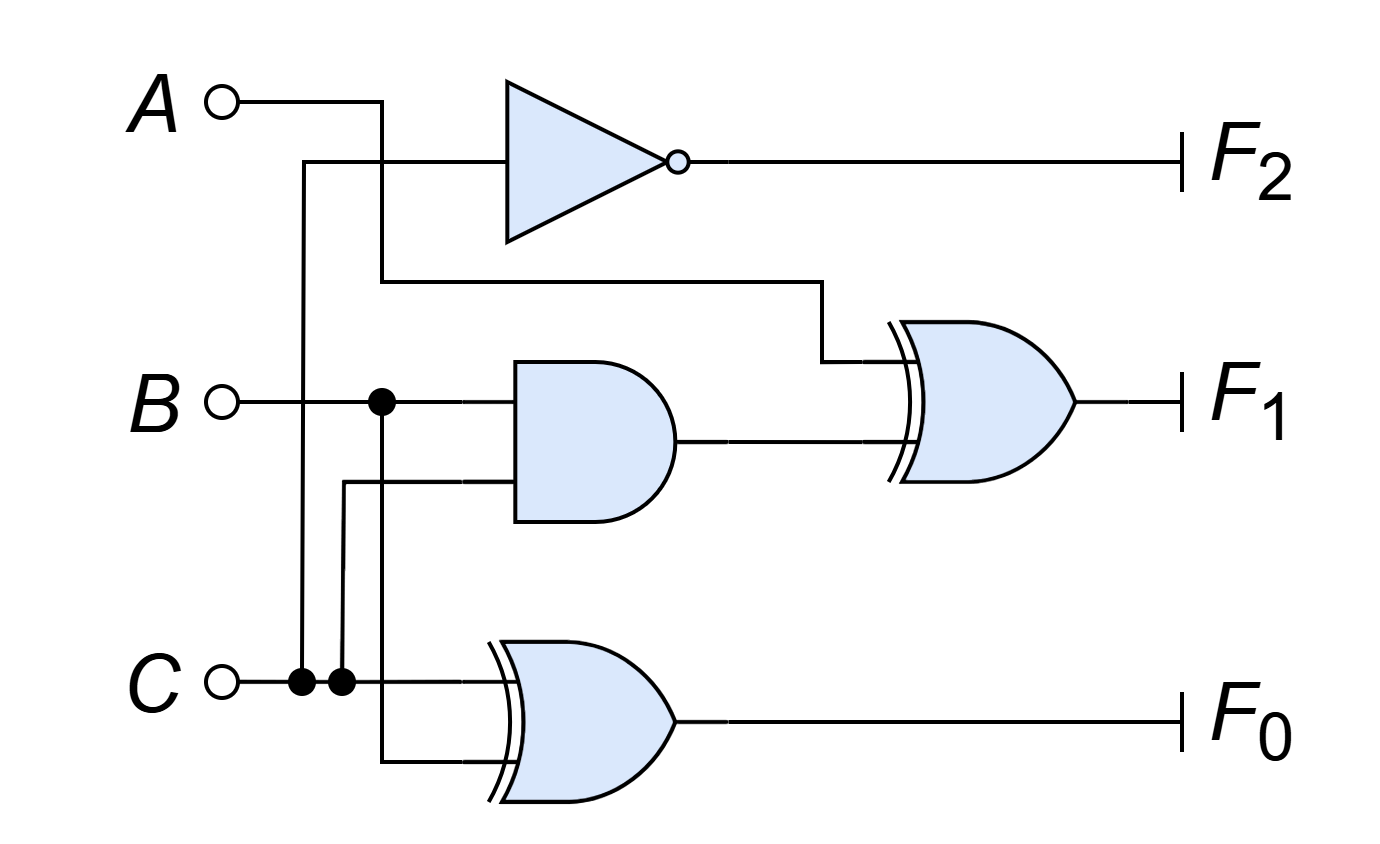
\includegraphics[scale=0.12]{Circuits/202409250229.png}
			}}\)
		}
		\quad
		\subfloat[真值表]{
			\belowrulesep=0pt
			\aboverulesep=0pt
			\label{Tab: Combinational Logic Circuit 1}
			\begin{tabular}{ccc|ccc}
				\toprule
				\(\symbf{A}\) & \(\symbf{B}\) & \(\symbf{C}\) & \(\symbf{F_0}\) & \(\symbf{F_1}\) & \(\symbf{F_2}\) \\
				\midrule
				0 & 0 & 0 & 0 & 0 & 1 \\
				0 & 0 & 1 & 0 & 1 & 0 \\
				0 & 1 & 0 & 0 & 1 & 1 \\
				0 & 1 & 1 & 1 & 0 & 0 \\
				1 & 0 & 0 & 1 & 0 & 1 \\
				1 & 0 & 1 & 1 & 1 & 0 \\
				1 & 1 & 0 & 1 & 1 & 1 \\
				1 & 1 & 1 & 0 & 0 & 0 \\
				\bottomrule
			\end{tabular}
		}
		\caption{组合逻辑电路实例 1}
	\end{figure}
	\begin{solution}
		根据逻辑门的运算规则,可得到
		\[
			\begin{cases}
				F_0 = A \oplus (B \cdot C) \\
				F_1 = B \oplus C \\
				F_2 = \overline{C}
			\end{cases}
		\]
		因此,该组合逻辑电路输出的真值表如表~\ref{Tab: Combinational Logic Circuit 1}~所示。
		可以看出,这个电路所实现的功能为 \((F_0F_1F_2)_2 = (ABC)_2 + 1\),这是一个 3-bit 二进制自增电路。
	\end{solution}
\end{example}

\begin{example}[1]
	分析如图~\ref{Fig: Combinational Logic Circuit 2}~所示的组合逻辑电路。
	\begin{figure}[!ht]
		\centering
		\subfloat[逻辑电路]{
			\label{Fig: Combinational Logic Circuit 2}
			\(\vcenter{\hbox{
				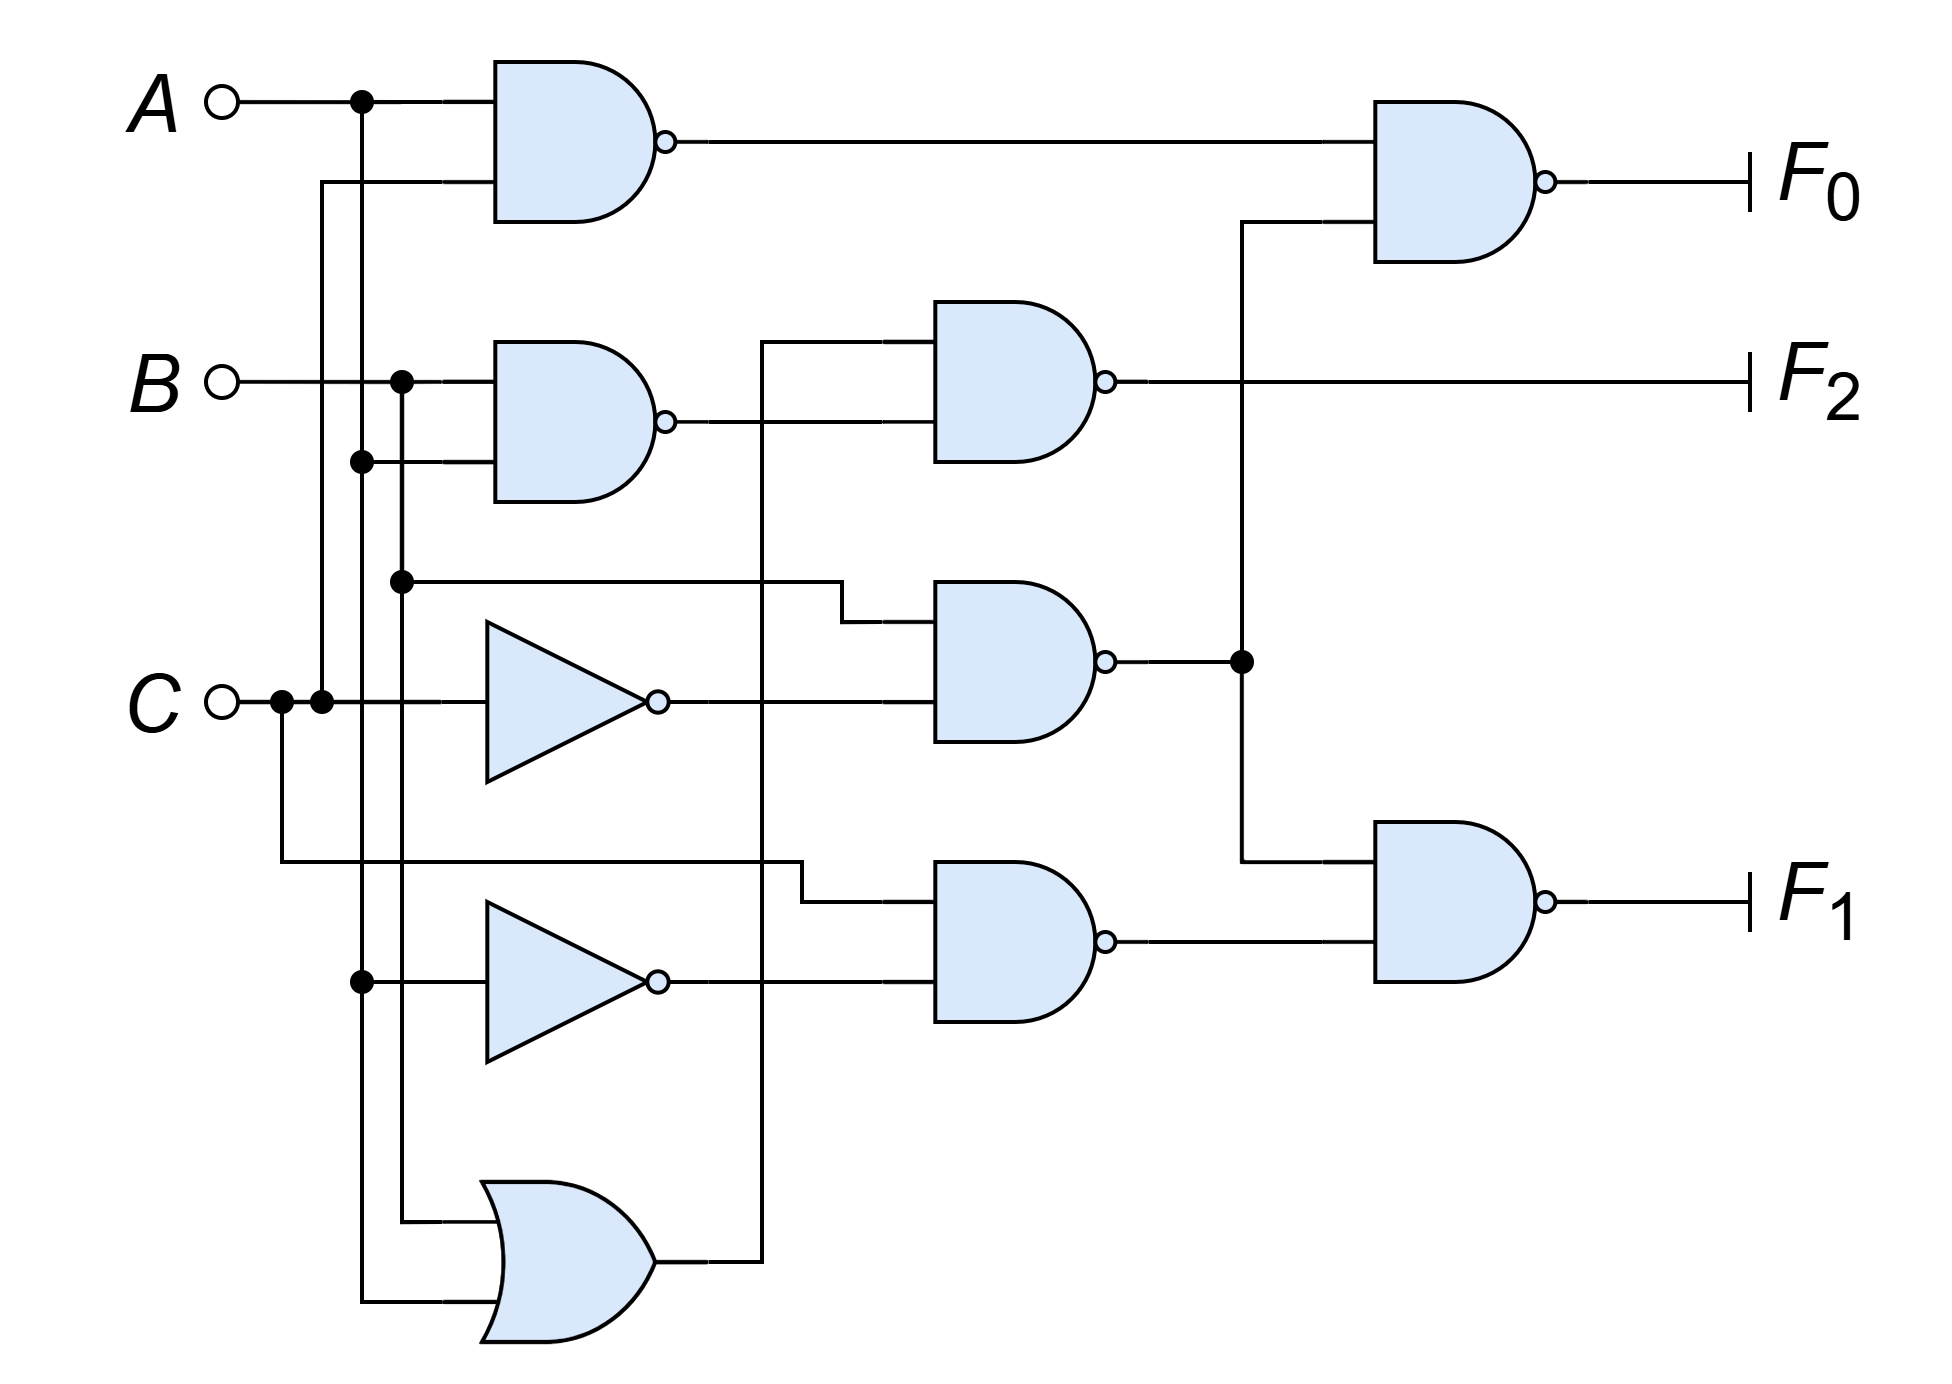
\includegraphics[scale=0.12]{Circuits/202409251632.png}
			}}\)
		}
		\quad
		\subfloat[真值表]{
			\belowrulesep=0pt
			\aboverulesep=0pt
			\begin{tabular}{ccc|ccc}
				\toprule
				\(\symbf{A}\) & \(\symbf{B}\) & \(\symbf{C}\) & \(\symbf{D}\) & \(\symbf{F_0}\) & \(\symbf{F_1}\) \\
				\midrule
				0 & 0 & 0 & 0 & 0 & 1 \\
				0 & 0 & 1 & 0 & 1 & 1 \\
				0 & 1 & 0 & 1 & 1 & 0 \\
				0 & 1 & 1 & 0 & 1 & 0 \\
				1 & 0 & 0 & 0 & 0 & 0 \\
				1 & 0 & 1 & 1 & 0 & 0 \\
				1 & 1 & 0 & 1 & 1 & 1 \\
				1 & 1 & 1 & 1 & 0 & 1 \\
				\bottomrule
			\end{tabular}
			\label{Tab: Combinational Logic Circuit 2}
		}
		\caption{组合逻辑电路实例 2}
	\end{figure}
	\begin{solution}
		根据逻辑门的运算规则,可得到
		\[
			\begin{cases}
				F_0 = \overline{\overline{AC} \cdot \overline{B\overline{c}}} \\
				F_1 = \overline{\overline{B\overline{C}} \cdot \overline{C\overline{A}}} \\
				F_2 = \overline{(A+B) \cdot \overline{AB}}
			\end{cases}
		\]
		因此,该组合逻辑电路输出的真值表如表~\ref{Tab: Combinational Logic Circuit 2}~所示,这是一个 Gray 码递增电路。
	\end{solution}
\end{example}

\subsubsection{组合逻辑电路的设计过程}

设计一个组合逻辑电路,需要将算法转化为二元逻辑的计算,化简后用逻辑电路结构实现。

\begin{example}[3]
	设计一个 2-bit 比较器。
	\begin{solution}
		2-bit 比较器的设计需求为:
		\begin{itemize}
			\item 功能:比较两个 2-bit 二进制数的大小;
			\item 输入:两个 2-bit 二进制数 \(A_1A_0\) 和 \(B_1B_0\);
			\item 输出:三个逻辑值 \(LT\)、\(EQ\) 和 \(GT\),分别表示 \(A < B\)、\(A = B\) 和 \(A > B\)。
		\end{itemize}
		用卡诺图表示出 \(LT\)、\(EQ\) 和 \(GT\) 的逻辑表达式如表~\ref{Tab: 2-bit Comparator}~所示,即知其两级与或表达式为
		\begin{align*}
			& LT = A_1'B_1 + A_1'A_0'B_0 + A_0'B_1B_0 \\
			& EQ = A_1'A_0'B_1'B_0' + A_1'A_0B_1'B_0 + A_1A_0'B_1B_0' + A_1A_0B_1B_0 \\
			& GT = A_1B_1' + A_1B_1'B_0' + A_1A_0B_0'
		\end{align*}
		其中 \(EQ\) 可以更简单地表示为
		\[
			EQ = \overline{A_1 \oplus B_1} \cdot \overline{A_0 \oplus B_0}
		\]
		或者利用另外两个输出的逻辑表达式,即
		\[
			EQ = \overline{LT + GT}
		\]
		将 \(LT\)、\(EQ\) 和 \(GT\) 的逻辑表达式转化为逻辑电路,即可得到 2-bit 比较器的设计。
	\end{solution}
	\begin{table}[!ht]
		\belowrulesep=0pt
		\aboverulesep=0pt
		\caption{2-bit 比较器设计的卡诺图}
		\label{Tab: 2-bit Comparator}
		\subfloat[\(LT\)]{
			\begin{tabular}{c|cccc}
				\toprule
				\(A_1A_0 \backslash B_1B_0\) & 00 & 01 & 11 & 10 \\
				\midrule
				00 &   & 1 & 1 & 1 \\
				01 &   &   & 1 & 1 \\
				11 &   &   &   &   \\
				10 &   &   & 1 &   \\
				\bottomrule
			\end{tabular}
		}
		\subfloat[\(EQ\)]{
			\begin{tabular}{c|cccc}
				\toprule
				\(A_1A_0 \backslash B_1B_0\) & 00 & 01 & 11 & 10 \\
				\midrule
				00 & 1 &   &   &   \\
				01 &   & 1 &   &   \\
				11 &   &   & 1 &   \\
				10 &   &   &   & 1 \\
				\bottomrule
			\end{tabular}
		}
		\subfloat[\(GT\)]{
			\begin{tabular}{c|cccc}
				\toprule
				\(A_1A_0 \backslash B_1B_0\) & 00 & 01 & 11 & 10 \\
				\midrule
				00 &   &   &   &   \\
				01 & 1 &   &   &   \\
				11 & 1 & 1 &   & 1 \\
				10 & 1 & 1 &   &   \\
				\bottomrule
			\end{tabular}
		}
	\end{table}
\end{example}


如上 4-bit 输入的逻辑运算已经比较复杂。对于更加复杂的逻辑运算,在处理中需要采取更多的技巧以简化运算,如:
\begin{itemize}
	\item 将输入变量分组,写成更简单的逻辑表达式的多级运算:
	\[
		f(A,B,C,\cdots) = F(g_1(A,B,\cdots),g_2(C,\cdots),\cdots)
	\]
	\item 将输入变量分离,写成更简单的逻辑表达式的分支计算:
	\[
		f(A,B,C,\cdots) = A \cdot g_1(B,C,\cdots) + \overline{A} \cdot g_2(B,C,\cdots)
	\]
	\item 从结构化表达式中找出重复的部分加以复用,简化逻辑电路。
\end{itemize} 
同时,还需要照应到实际的功耗、性能、面积等要求。

\subsubsection{组合逻辑电路的评价指标}

评价逻辑电路的主要指标包括:
\begin{itemize}
	\item 稳态因素:
	\begin{itemize}
		\item \textbf{逻辑电平}:逻辑电路的输入和输出电平高低;
		\item \textbf{噪声容限}:逻辑电路抵抗噪声的能力;
		\item \textbf{静态功耗}:逻辑电路在稳态工作时的功耗,主要与电路的 \(V_{CC}\) 有关;
		\item \textbf{面积}:逻辑电路的物理尺寸;
		\item \textbf{扇出系数}:逻辑门的输出能够驱动的输入数量。
	\end{itemize}
	\item 动态因素:
	\begin{itemize}
		\item \textbf{传输延迟}和\textbf{时钟频率}:逻辑电路的输入到输出的延迟时间;
		\item \textbf{时序容限}:逻辑电路的输入信号的时序要求;
		\item \textbf{动态功耗}:逻辑电路在工作时的功耗,主要与电路的切换频率有关;
		\item \textbf{噪声}:逻辑电路在工作时产生的噪声。
	\end{itemize}
\end{itemize}

\subsubsection{组合逻辑电路的设计实例}

\paragraph{编码器(Encoder)和译码器(Decoder)}

用 \(m\) 个二进制位对 \(n \le 2^m\) 个输入信号进行编码,得到 \(m\) 位二进制代码的电路,称为 \,\(\mboba{2^m - m}\)\,\tboba{线编码器}。

\begin{example}[3]
	设计一个 \(4-2\) 线编码器用作抢答器,其中每个抢答按钮按下时对应输入信号为1,其余输入信号为0。
	\begin{solution}
		4 个输入信号的抢答器的真值表如表~\ref{Tab: 4-2 Encoder}~所示\footnote{
			由于编码器的输入信号类型数最多为输出信号所能表示的最大数值,其必定要用\textbf{无关项}的形式归总一些设计之外的情况。考虑到输出信号的唯一性,表中无关项的分布不是对称的。
		},容易得到其逻辑表达式为
		\begin{align*}
			& Y_0 = A_3 + A_1 \\[-3pt]
			& Y_1 = A_3 + A_2
		\end{align*}
		该编码器的设计如图~\ref{Fig: 4-2 Encoder}~所示。

		但是,这个编码器不能满足抢答器的优先要求。为了实现优先级,可以将输入信号的优先级从高到低排列,然后将优先级高的输入信号的输出信号设为1,优先级低的输入信号的输出信号设为0。具体的电路设计略。
	\end{solution}
	\begin{figure}[!ht]
		\belowrulesep=0pt
		\aboverulesep=0pt
		\centering
		\subfloat[真值表]{
			\label{Tab: 4-2 Encoder}
			\begin{tabular}{cccc|cc}
				\toprule
				\(A_3\) & \(A_2\) & \(A_1\) & \(A_0\) & \(Y_1\) & \(Y_0\) \\
				\midrule
				\(\times\) & \(\times\) & \(\times\) & 1 & 0 & 0 \\
				\(\times\) & \(\times\) & 1 & 0 & 0 & 1 \\
				\(\times\) & 1 & 0 & 0 & 1 & 0 \\
				1 & 0 & 0 & 0 & 1 & 1 \\
				\bottomrule
			\end{tabular}
		}
		\quad
		\subfloat[逻辑电路]{
			\label{Fig: 4-2 Encoder}
			\(\vcenter{\hbox{
				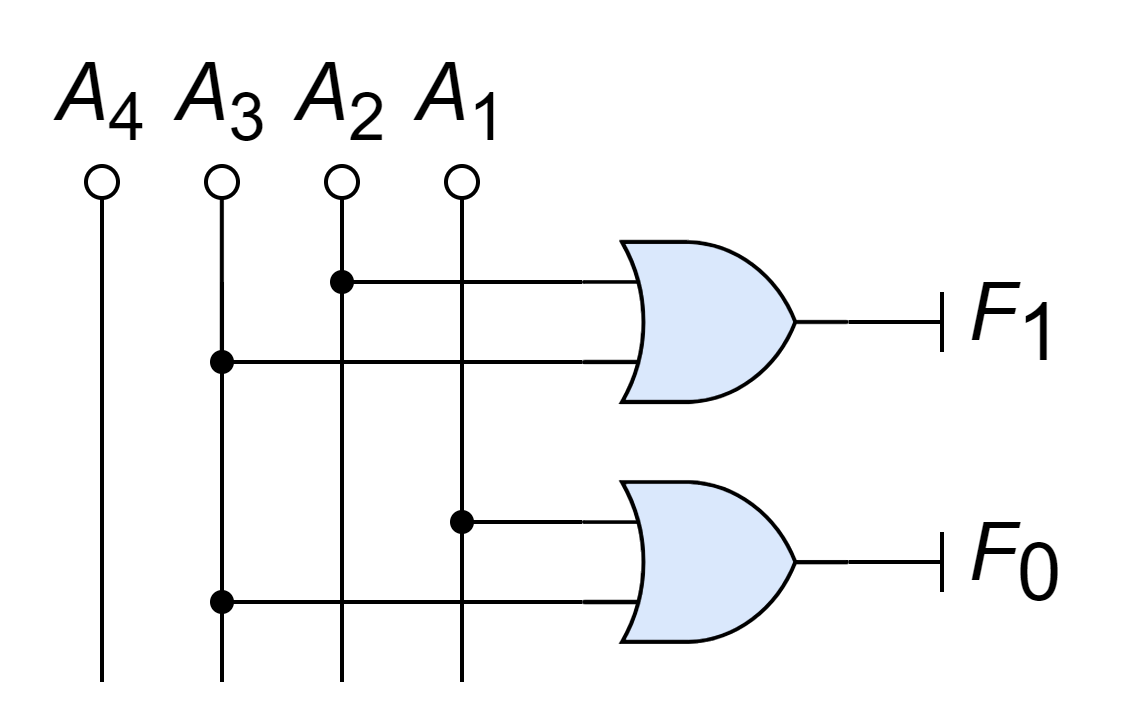
\includegraphics[scale=0.12]{Circuits/202409262050.png}
			}}\)
		}
		\caption{\(4-2\) 线编码器设计}
		\vspace{-2em}
	\end{figure}
\end{example}

译码是编码的逆过程,即将编码后的信号转换为原始信号。用 \(n\) 个二进制位对 \(m \le log_2 n\) 个输入信号进行译码,得到 \(n\) 位二进制代码的电路,称为 \,\(\mboba{log_2 n - n}\)\,\tboba{线译码器}。

\paragraph{多路选择器(Multiplexer,MUX)}

用 \(n\) 个控制信号对 \(2^n\) 个输入信号进行选择,得到一个输出信号的电路,称为 \,\(\mboba{2^n : 1}\)\,\tboba{多路选择器}。

\paragraph{加法器}

用于实现二进制数的加法运算。

\begin{example}[3]
	设计一个 4-bit 全加器电路。
	\begin{solution}
		1-bit 全加器有 3 个输入信号( \(A\)、\(B\) 和进位信号 \(C_\mathrm{in}\))、2 个输出信号(本位的和 \(S\) 、进位输出信号\(C_\mathrm{out}\)。则
	\end{solution}
\end{example}


%----------------------------------------------------------
\end{document}
